\chapter{Quantum-Thermodynamics from a Unitary Perspective}
\label{sec:therm_results}
After the precision studies of \cref{sec:hopsvsanalyt,sec:prec_sim} we
turn to applications of the formalism developed in \cref{chap:flow}
that are related to thermodynamic questions\fixme{add some
  citations}. Because the NMQSD HOPS provide access to the global
unitary dynamics of system (working medium) and bath, it is
predestined to be put to use in this field.

We will begin with some theoretical notions in \cref{sec:basic_thermo}
and then continue to apply them to some very simple cases in
\cref{sec:singlemod,sec:otto}.

\section{Some Theoretical Notions}
\label{sec:basic_thermo}
The field of quantum thermodynamics is a complex one and we will
restrict the account given here to the minimum required for the
presentation of the subsequent results. A comprehensive account can be
found in
\cite{Binder2018,Kurizki2021Dec,Talkner2020Oct,Vinjanampathy2016Oct}.

Many central questions in thermodynamics are concerned with energy
extraction from macroscopic systems. These questions can be framed in
operational terms that don't require a specific definition of heat and
just rely on the energy change in the total system or its
constituents. These quantities are now accessible to us in a rather
general setting, making issues related energy extraction a prime
application for our method.

Here, we will focus on two closely related problems. The first is
concerned with how much energy can be extracted through a unitary
transformation from a single infinite thermal bath coupled to an
arbitrary finite dimensional working medium. We call this energy
\emph{ergotropy}\footnote{see \cref{eq:ergo_def} for a more precise
  definition}.

In Thermodynamics the second law tells us that in this setting no
energy can be extracted in a periodic manner.  It turns out that in
the full quantum case such a result can be obtained by studying bounds
on the ergotropy of the system as is done in
\cref{sec:ergo_general}. Remarkably these bounds will turn out to be
finite. We will review a general bound for single bath systems in
\cref{sec:ergoonebath} and study an explicit calculation for a simple
case in \cref{sec:explicitergo}. The latter study will elucidate under
which conditions we may expect the bound to be tight.

The second problem is a generalization of the above considerations to
systems coupled to multiple baths of different temperature. Here,
naturally, the ergotropy is generally not bounded. However, there is a
limit to how efficiently energy can be extracted. To quantify
efficiency one has to introduce a notion of thermodynamic
cost. Traditionally this is the entropy production or the amount of
``waste heat'' that is being shed into the cold reservoir instead of
being extracted as work. Both quantities require a proper definition,
that can usually be given, but which is not unique due to the issue
of finite interaction energy\footnote{see the discussion in
  \cref{chap:intro}}.

Nevertheless, when the system is periodically modulated so that the
interaction energy expectation value is periodic, we can clearly
divide system and bath energies. In this case it becomes clear, that
we can define the efficiency for a system with a hot and a cold bath
as
\begin{equation}
  \label{eq:efficiency_definition}
  η = \frac{Δ\ev{H_{\bath}}_{\mathrm{cyc},c}}{Δ\ev{H}_{\mathrm{cyc}}},
\end{equation}
where \(Δ\ev{H_{\bath}}_{\mathrm{cyc},c}\) is the cold bath energy change
over one cycle and \({Δ\ev{H}_{\mathrm{cyc}}}\) is the total energy
change over one cycle.

In \cref{sec:operational_thermo} a Gibbs like inequality for an
arbitrary number of baths is derived as a very slight generalization
of the derivation in~\cite{Kato2016Dec}. The left hand side of this
inequality can be associated with a thermodynamic cost that should be
minimized for optimal efficiency.

\subsection{The Ergotropy of Open Quantum Systems}
\label{sec:ergo_general}
The ergotropy of a quantum system is defined\fixme{mention paper that
  uses ergo for heat}
as~\cite{Binder2018}
\begin{equation}
  \label{eq:ergo_def}
  \ergo{ρ} = \max_{U\,\text{unitary}}\tr[\qty(ρ - UρU^\dag) H],
\end{equation}
which is the maximal energy that can be extracted from a system
through cyclic modulation of the Hamiltonian \(H\). A state is called
passive iff the maximizing \(U\) \cref{eq:ergo_def} is the identity
\(\id\) and its ergotropy vanishes. In other words, a state is passive
if it's energy can not be reduced through unitary transformations.

The immediate appeal of this quantity for later applications is, that
it is formulated with respect to the full unitary dynamics which is
accessible to us through HOPS.

A passive state \(ρ_P\) is always diagonal in the eigenbasis of \(H\)
and its eigenvalues satisfy the following ordering
condition~\cite{Lenard1978Dec}
\begin{equation}
  \label{eq:passive_diag}
  ρ_{p}=∑_{j=1}^{n} \lambda_{j}|j\rangle\langle j|, \quad E_{j} \leq E_{j+1}, \quad \lambda_{j+1} \leq \lambda_{j},
\end{equation}
where \(n<∞\) is the Hilbert space dimension. This condition is both
necessary and sufficient. Examples of passive states are the state of
the micro-canonical ensemble or Gibbs states. Gibbs states are further
distinguished by additional features as described
in~\cite{Lenard1978Dec}, which can be connected to formulations of the
zeroth and second laws of thermodynamics.

One of these properties is complete passivity. Completely passive
states remain passive under the transformation \(ρ\to\otimes^Nρ\) (and
an \(N\)-fold sum of the Hamiltonian) for finite \(N\). Therefore no
energy can be extracted from multiple identical systems in equilibrium
at the same temperature.  For finite dimensional systems, the complete
passivity even implies the the Gibbs state.

The open-systems case differs as here a ``small'' system is coupled to
a bath of infinite size. If the system state is not a Gibbs state, the
whole system becomes non-passive, even if the system state is passive
with respect to the system Hamiltonian\footnote{for example being the
  ground state}.

For systems of infinite size, states fulfilling the
Kubo–Martin–Schwinger (KMS) condition have been proposed as the
generalizations of Gibbs states, having similar properties. Under some
conditions passivity implies the KMS condition. These conditions are
related to the fact that KMS states are not necessarily
unique~\cite{Binder2018,Pusz1978Oct}.

The KMS condition is stated for two arbitrary observables \(A,B\) and
\(F_{AB}(t)=\tr[ρ_βA(t)B(0)]\) (Heisenberg picture,
\(A(t)=\eu^{\iu H t}H\eu^{-\iu H t}\)) as
\begin{equation}
  \label{eq:kmscond}
  F_{AB}(-t) = F_{BA}(t-\iu β)
\end{equation}
by virtue of analytic continuation and does not rely on a concrete
expression of the state \(ρ_{β}\) which may not exist in the
traditional sense.

For example, the Carnot efficiency bound can be proven
rigorously~\cite{Pusz1978Oct} for two KMS states of different
temperatures.

In the following we will restrict our discussions to finite
dimensional systems, taking the thermodynamic limit when it is
appropriate. KMS states only enter the NMQSD/HOPS formalism
indirectly, as they predict the expression for negative frequency part
of the finite temperature spectral density. Due to the formulation of
the NMQSD which only relies on bath correlation functions, the problem
of non-existing states is circumvented.

In fact, we see in \cref{fig:bcf_approx} that the BCF of an infinite
bath can be approximate very well by a finite number of evenly spaced
oscillators for finite times\footnote{Finite times include the
  lifetime of the universe.}. For such a bath the thermal state is
trace class, albeit not finite dimensional. However, for finite
temperature the individual oscillator Hilbert spaces may be suitably
truncated making the whole bath finite dimensional, justifying our
finite dimensional treatment in the following.
\begin{figure}[htp]
  \centering
  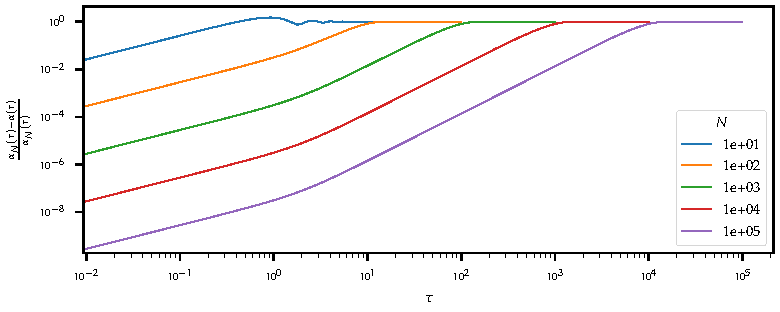
\includegraphics{figs/misc/bcf_approx}
  \caption{\label{fig:bcf_approx} An ohmic BCF with \(ω_{c}=η=1\)
    approximated by the BCF of linearly spaced oscillators. The figure
    plots the relative difference between an approximation with \(N\)
    oscillators and the exact BCF over time. An order of magnitude
    more oscillators give an approximation which is valid for an order
    of longer dimensionless period.}
\end{figure}

The Hamiltonian of a finite dimensional system is bounded and
therefore the ergotropy of such a system is finite. However, in the
following we will find that the ergotropy cannot even be made
arbitrarily large by enlarging the bath.


\subsection{Quantum Friction}
\label{sec:quantum_friction_theory}
A simple application of the notion ergotropy is an explanation for so
called \emph{quantum
  friction}~\cite{Binder2018,Mukherjee2020Jan}. This is an
unfortunate term. From it one would expect that quantum friction has
some connection to dissipation. In fact the reverse is true in most
cases where it is a concept applied to the reduced state of the
system.

Consider a modulated open quantum system.  The buildup of energy basis
coherence in the system state makes it non-passive.  Thus additional
energy which cannot be extracted by modulating of the energy level
gaps of the system\footnote{This is the usual mechanism of energy
  extraction in a quantum Otto
  cycle~\cite{Geva1992Feb}.}~\cite{Kurizki2021Dec} is tied up in the
system state, reducing power output.  The reduction of power output in
through quantum coherence general has been termed quantum
friction. However, the occurrence of coherence is not necessarily
detrimental\fixme{do more research on that.refer to simulations}, if
the system is restored to a diagonal state\footnote{Shortcuts to
  adiabaticity, see for example~\cite{Chen2010Feb}.}.

\subsection{The Ergotropy of Finite Systems Coupled to a Thermal Bath}
\label{sec:ergoonebath}
We have argued above that Gibbs states play a special role. Here, we
explore the ergotropy of such a state to an arbitrary finite
dimensional systems. Our goal will be to ensure thermodynamic
consistency of the global unitary dynamics of such a system.

Let us consider models with the Hamiltonians
\begin{equation}
  \label{eq:simple_bath_models}
  H = \id_\sys\otimes H_\bath + H_\sys\otimes \id_\bath,
\end{equation}
where the system \(\sys\) is finite dimensional and \(H_\bath\) may be
chosen arbitrarily. Let the initial state of the system be
\begin{equation}
  \label{eq:simple_initial_state}
  ρ=ρ_\sys\otimes τ_β,
\end{equation}
where \(τ_β=\eu^{-β H_\bath}/Z\) is a Gibbs state and \(ρ_\sys\) is
arbitrary.

An interesting question is whether the ergotropy of such a state is
finite. This amounts to the formulation of the second law: ``No energy
may be extracted from a single bath in a cyclical manner''.
For systems obeying GKSL dynamics connected to a KMS state heat bath,
thermodynamic laws can be derived in certain situations\footnote{very
  slow or very fast modulation of the system
  hamiltonian}\cite{Binder2018}, which imply the answer ``yes'' for the
above questions. In the non-Markovian case, those arguments do not
hold anymore.

For finite dimensional baths, we always have finite ergotropies, as
their Hamiltonians are bounded. In the infinite dimensional case, we
may expect that the ergotropy is still finite for some models, as long
as the energies of the thermal states for those models is finite. This
assumption breaks down when we consider infinite baths, whose thermal
energy is unbounded even for finite temperatures. In terms of finite
baths we may ask whether the ergotropy of the system can be made
arbitrarily large by enlarging the bath.

There is a simple and general argument that provides and upper bound
on the ergotropy of states of the form~\cref{eq:simple_initial_state}
based on the special form of Gibbs states and relative entropy. The
latter quantity allows the application of quantum informational tools,
even in the presence of infinite baths if we are careful in taking
limits.

The derivation of the following bound is adapted
from~\cite{Biswas2022May,Alicki2013Apr,Lobejko2021Feb}. We limit
ourselves to finite dimensional problems for now.  As unitary
transformations leave the entropy invariant
(\(\tr[ρ\ln(ρ)] = \tr[ρ_P\ln(ρ_P)]\)), we have for an arbitrary
\(β > 0\) and \(ρ_β=\exp(-βH)/Z\), \(Z=\tr[\exp(-βH)]\)
\begin{align}
    \ergo{ρ} &= E(ρ) - E(ρ_P) = \tr[(ρ-ρ_P) H]\nonumber\\
             &= -\frac{1}{β}\tr[(ρ-ρ_P)
               \qty(\ln(ρ_β) + \ln(Z))] \nonumber\\
             &= -\frac{1}{β}\tr[(ρ-ρ_P) \ln(ρ_β)]\nonumber\\
             &=\frac{1}{β}\qty{\tr[ρ\qty(\ln(ρ) - \ln(ρ_β))] -
               \tr[ρ_P\qty(\ln(ρ_p) - \ln(ρ_β))]}\nonumber\\
             &\equiv\frac{1}{β}\qty[\qrelent{ρ}{ρ_β} - \qrelent{ρ_P}{ρ_β}]\label{eq:ergo_entro},
\end{align}
where we have used \(\tr[ρ]=\tr[ρ_P]=1\).

The relative entropies
appearing in \cref{eq:ergo_entro} are always finite, as \(ρ\) is
finite-dimensional and \(ρ_β\) has full rank.  As energy is minimized
by a Gibbs state when keeping the entropy fixed, we find an upper
bound on the ergotropy by replacing \(ρ_P\to ρ_{β^\ast}\) in
\cref{eq:ergo_entro} where
\(S(ρ_{β^\ast})=S(ρ)\)~\cite{Alicki2013Apr}.

By choosing the temperature in \cref{eq:ergo_entro} accordingly, we
arrive at
\begin{equation}
  \label{eq:ergo_bound_single}
  \ergo{ρ} \leq \frac{1}{β^\ast}\qrelent{ρ}{ρ_{β^\ast}}.
\end{equation}
This bound can be saturated for states which are a permutation of a
thermal state, as their corresponding passive state is the thermal
state.

For our setting in
\cref{eq:simple_bath_models,eq:simple_initial_state} we find a still
better way to bound the ergotropy and fix the
temperature~\cite{Lobejko2021Feb}. Substituting \(ρ\to ρ \otimes τ_β\)
in \cref{eq:ergo_entro} we obtain
\begin{equation}
  \label{eq:thermo_ergo_bound}
  \begin{aligned}
  \ergo{ρ\otimes τ_β} &= \frac{1}{β}
  \qty[\qrelent{ρ\otimes τ_β}{ρ_β\otimes τ_β} - \qrelent{(ρ\otimes
                        τ_β)_P}{ρ_β\otimes τ_β}]\\
    &=\frac{1}{β}
  \qty[\qrelent{ρ}{ρ_β} - \qrelent{(ρ\otimes τ_β)_P}{ρ_β\otimes
      τ_β}] \leq \frac{1}{β} \qrelent{ρ}{ρ_β},
  \end{aligned}
\end{equation}
where the positivity of relative entropy has been used.

Remarkably, the bound \cref{eq:thermo_ergo_bound} only depends on the
system state and ``inherits'' the temperature of the bath. For any
\(\dim[τ_β] = N\gg 1\) the bound stays valid and independent of any
bath properties except the temperature. It is therefore reasonable to
expected that it is also valid for an infinite bath.

Interestingly, a saturation of \cref{eq:thermo_ergo_bound} is achieved
in~\cite{Skrzypczyk2014Jun} with a continuous qubit
bath. In~\cite{Lobejko2021Feb} a more generic argument is made in a
similar setting. Both propose concrete protocols within the bounds of
thermal operations and by considering explicit work reservoirs. In
\cref{sec:explicitergo} we will provide another example which
asymptotically saturates the bound.

For the term \(\qrelent{(ρ\otimes τ_β)_P}{ρ_β\otimes τ_β}\) to vanish
in \cref{eq:thermo_ergo_bound}, the state bath and system should be as
close to the product thermal state as possible and so the bath state
should not change too much. This is achievable with a continuous
infinite size bath.

A corollary of \cref{eq:thermo_ergo_bound} is the Clausius form of the
second law. By setting the system Hamiltonian to \(α \id\) in the
above discussion the ergotropy becomes the change of bath energy
\begin{equation}
  \label{eq:ergo_bath_change}
  \begin{aligned}
    \ergo{ρ} &= \max_{U\,\text{unitary}}\tr[\qty(ρ - UρU^\dag)
               (α\id\otimes H_\bath)] \\
             &=\max_{U\,\text{unitary}}\tr_\bath\qty[\qty(\tr_\sys[ρ-UρU^\dag])
               H_\bath]\\
             &\equiv\max_{U\,\text{unitary}}ΔE_\bath\leq
               β^{-1}\qrelent{ρ}{\frac{\id_N}{N}}=β^{-1}\pqty{\log(N) - S(ρ)}
               \leq β^{-1}\log(N),
  \end{aligned}
\end{equation}
where \(N\) is the system dimension and \(α\) is arbitrary. No finite
amount of energy may therefore be extracted from the bath in a
periodic manner. If it were possible to extract a constant positive
amount of energy from the bath per cycle, \cref{eq:ergo_bath_change}
would be breached in finite time.


\subsection{The Ergotropy of a Two
  Level System and a Bath of Identical Oscillators}
\label{sec:explicitergo}
Before retreating to numerics to explore the bound from
\cref{sec:ergoonebath}, we will treat an illustrative example and
explicitly calculate the ergotropy for a simple model. This allows us
to see an indication how tight the bound can be.

Consider a two dimensional system connected to a bath of identical
oscillators. Throughout we will set the zero-point energy of the
oscillators to zero, meaning that \(H=ωa^\dag a\) for a single
harmonic oscillator with the usual annihilation operator \(a\).

Let us choose \(H_S=α\id_N\) as in \cref{eq:ergo_bath_change} for
simplicity, where \(α\) is an arbitrary energy scale. The ergotropy is
then equal to the maximal energy reduction of the bath under arbitrary
cyclic modulation.

The bound \cref{eq:thermo_ergo_bound} further simplifies to
\begin{equation}
  \label{eq:thermo_ergo_bound_specific}
  \ergo{ρ\otimes τ_β} \leq \frac{1}{β} \qty[\ln(N) - S(ρ)],
\end{equation}
where \(S(ρ)=-\tr[ρ\ln(ρ)]\).  For a pure state
\cref{eq:thermo_ergo_bound_specific} is maximal and we therefore
choose \(ρ=\ketbra{0}\) as an arbitrary pure state basis state of the
two level system. The state \(\bra{1}\) is the second basis state,
orthogonal to \(\ket{0}\).

If we take the system to be a qubit, the right hand side of
\cref{eq:thermo_ergo_bound_specific} is the Landauer bound
\(β^{-1}\ln2\). Therefore, upon saturation of the bound
\cref{eq:thermo_ergo_bound_specific} we can extract enough energy from
the bath to erase one bit in a system of the same temperature as the
bath. Indeed, owing to \cref{eq:thermo_ergo_bound_specific} the closer
the qubit state is to the infinite temperature (erased) state the more
certain we are, that we have extracted the maximum energy out of the
bath.

\paragraph{One Oscillator}
As a demonstration of the general program, let us first discuss the
ergotropy of a single harmonic oscillator with frequency \(ω\) as a
bath.  The initial state is given by
\begin{equation}
  \label{eq:onehoinit}
  ρ_{0} = ∑_{n=0}^{∞} \underbrace{Z^{-1}\eu^{-βωn}}_{λ_{0,n}} \ketbra{{0,n}},
\end{equation}
where \(Z=Z_{1}=\frac{1}{1-\eu^{-βω}}\) is the partition sum of one
bosonic mode with frequency \(ω\).

In contrast to the state characterized by \cref{eq:passive_diag} we
only fill every second level with \cref{eq:onehoinit}. To construct a
corresponding passive state\footnote{Due to the degeneracy of the
  system Hamiltonian, the passive state is not unique.} we have to
construct a sequence \(λ_{i},\, i \in \NN_{0}\) out of the weights
\(λ_{0,n}\) such that \(λ_{i}\geq λ_{j}\) for \(i\leq j\) and a
sequence of states \(\ket{j}\) so that for \(H\ket{j} = E_{j}\ket{j}\)
we have \(E_{i}\leq E_{j}\) for \(i\leq j\). The passive state and its
corresponding energy is then
\begin{equation}
  \label{eq:specific_passive_state}
  \begin{aligned}
    ρ_{p} &= ∑_{i} λ_{i} \dyad{i} & E_{p} &= ∑_{i} λ_{i}E_{i}.
  \end{aligned}
\end{equation}

In the present case, this is easily done by defining \(λ_{i}=λ_{0,i}\)
and
\begin{equation}
  \label{eq:state_enumeration_single}
  \ket{i} =
  \begin{cases}
    \ket{0, i/2} & i\text{ even} \\
    \ket{1, (i - 1) / 2} & i\text{ odd}. \\
  \end{cases}
\end{equation}

Thus, we find a passive state
\begin{equation}
  \label{eq:one_ho_pass}
  ρ_{p} = \frac{1}{Z} \qty[∑_{i} \eu^{-2i βω} \ketbra{0, i} +
  \eu^{-(2i + 1) βω} \ketbra{1, i}].
\end{equation}

The corresponding energy difference \(\ev{H (ρ_{0} - ρ_{p})}\) works
out to be
\begin{equation}
  \label{eq:one_ho_ergo}
  \mathcal{W} = ω\qty(\frac{1}{\eu^{βω} - 1} - \frac{1}{\eu^{2βω} - 1}) = ω \frac{\eu^{-β ω} - \eu^{-2 β ω}}{1-\eu^{-β
      ω}-\eu^{-2 β ω} + \eu^{-3 β ω}} \xrightarrow{βω
    \rightarrow ∞} \frac{ω}{\eu^{βω} - 1}.
\end{equation}

For low temperatures or large frequencies, the ergotropy of the
oscillator is just its mean thermal energy \(ω\bose(ωβ)\). In the
opposite limit we find \(\mathcal{W} = \frac{1}{7β}< β^{-1}\ln(2)\)
verifying the bound derived in \cref{sec:ergoonebath}.

\paragraph{Many Oscillators}
For the case of \(N>1\) oscillators with frequency \(ω\) the initial
state is
\begin{equation}
  \label{eq:manyhoinit}
  ρ_{0} = ∑_{\vb{n}\in\ZZ_{0}^{n}} \underbrace{Z^{-1}\eu^{-βω\abs{\vb{n}}}}_{λ_{0,\vb{n}}} \ketbra{{0,\vb{n}}},
\end{equation}
with the \(n_{i}=(\vb{n})_{i}\) labeling the state of the \(i\)th
oscillator and \(\abs{\vb{n}}=∑_{i=1}^{N}n_{i}\) and \(Z=Z_{1}^{N}\).

In this case we again call the ordered sequence of weights \(λ_{i}\),
but its construction is somewhat more complicated and we will refrain
from doing so here explicitly.  Instead we take an enumeration of
state labels \(\{\vb{n}^{i}\}_{i\in\NN_{0}}\) such that
\(i<j \implies m_{i} \leq m_{j}\) with
\(m_{i}\equiv\abs{\vb{n}^{i}}\). The energies of the states
\(\ket{k,\vb{n}^{i}}\) evaluate to \(E_{k, i} = ω m_{i}\) and the
initial weights to \(λ_{0,i}=Z^{-1}\eu^{-βω m_{i}},\,λ_{1,i}=0\).

The required enumeration of states and energies is then
\begin{equation}
  \label{eq:many_enum}
  \begin{aligned}
  \ket{i} &=
  \begin{cases}
    \ket{0, m_{i/2}} & i\text{ even} \\
    \ket{1, m_{(i-1)/2}} & i\text{ odd}
  \end{cases},
    & E_{i} &= ω m_{\lfloor{i/2}\rfloor}
  \end{aligned}
\end{equation}
and the enumeration of weights is \(λ_{i} = λ_{0,i} =Z^{-1}\eu^{-βω m_{i}}\).


The corresponding passive state energy will be
\begin{equation}
  \label{eq:many_ho_pass}
  E_{p} = \frac{ω}{Z} ∑_{i=0}^{∞} m_{i} \pqty{\eu^{-ωβ m_{2i}} + \eu^{-ωβ m_{2i+1}}}.
\end{equation}

For each value of \(m\) of \(\qty{m_{k}}\) there are
\(G_{m}^{N} = \binom{N+m-1}{N-1}\) sequence elements \(m_{i}\) with
\(m_{i}=m\).  We define the sequence \(\qty{x_{m}}_{m\in\NN_{0}}\) so
that \(x_{m}=G^{N+1}_{m}=\binom{N+m}{m}\) denotes the index \(i\)
until which \(m_{i}\) has the value \(m\). Likewise
\(\qty{y_{m}}_{m\in\NN_{0}}\) is defined so that
\(y_{m}=\big\lceil G^{N+1}_{m}/2\big\rceil\) denotes the index \(i\)
until which \(m_{2i}\) retains the value \(m\). When using the floor
instead of ceil in the definition of \(y_{m}\) we find that this
sequence \(\qty{z_{m}}_{m\in\NN_{0}}\) fulfills the same purpose but
for \(m_{2i+1}\).

Now, let
\begin{equation}
  \label{eq:deltas}
  \begin{aligned}
    Δ^{e}_{m,m} &= y_{m}-x_{m-1}
                  =\left\lceil\frac{G^{N+1}_{m}}{2}\right\rceil -
                  G^{N+1}_{m-1} & Δ^{e}_{m,m+1} &= x_{m}-y_{m}
                  =G^{N+1}_{m} - \left\lceil\frac{G^{N+1}_{m}}{2}\right\rceil\\
  Δ^{o}_{m,m} &= z_{m}-x_{m-1}
                  =\left\lfloor\frac{G^{N+1}_{m}}{2}\right\rfloor -
                  G^{N+1}_{m-1} & Δ^{o}_{m,m+1} &= x_{m}-z_{m}
                  =G^{N+1}_{m} - \left\lfloor\frac{G^{N+1}_{m}}{2}\right\rfloor.
  \end{aligned}
\end{equation}

The \(Δ^{e}_{m,k}\) denotes the number of indices \(i\) where
\(m_{i}=m\) and \(m_{2i}=k\) and the \(Δ^{e}_{m,k}\) have the same
function, but for \(m_{2i+1}\).
The equations \cref{eq:deltas} lists explicit formulas only for the
case where the difference is at most one, but this is sufficient for
the estimate we will discuss now.

We find
\begin{equation}
  \label{eq:manhoergoestimate}
  \begin{aligned}
    E_{p} &\geq \frac{ω}{Z} ∑_{m=1}^{∞} m \bqty{\eu^{-m
            ωβ}\pqty{Δ^{o}_{m,m} + Δ^{e}_{m,m}} + \eu^{-(m+1)
            ωβ}\pqty{Δ^{o}_{m,m+1} + Δ^{e}_{m,m+1}}} \\
          &= \frac{ω}{Z} ∑_{m=1}^{∞} m\eu^{-m
            ωβ} \bqty{G^{N+1}_{m} - 2 G^{N+1}_{m-1} +
            G^{N+1}_{m}\eu^{-ωβ}}\\
          &= \frac{ω}{Z} ∑_{m=1}^{∞} m\eu^{-m
            ωβ} \bqty{G^{N}_{m} - G^{N+1}_{m-1} + G^{N+1}_{m}\eu^{-ωβ}},
  \end{aligned}
\end{equation}
where we have used that all summands are nonnegative and we could
therefore obtain a lower bound on the passive energy by dropping all
terms where the difference between \(m_{i}\) and \(m_{2i}\,,m_{2i+1}\)
is greater than one. The terms for which this is true will have large
values of \(m\) and will further be suppressed by a factor of
\(\eu^{-kωβ}\) (\(k\geq 2\)) so one might expect this bound to be
tight for large \(ω\) and large \(N\).

We can evaluate \cref{eq:manhoergoestimate} further by noting
\begin{equation}
  \label{eq:many_ho_orig_energy}
  E_{0} = \tr[ρ_{0}H]
  = \frac{1}{Z} ∑_{\vb{n}\in\NN_{0}^{N}} ω\abs{\vb{n}}
  \eu^{-\abs{\vb{n}}ωβ}
  = \frac{ω}{Z} ∑_{m=1}^{∞} m G^{N}_{m}\eu^{-mωβ}
\end{equation}
and also
\begin{equation}
  \label{eq:manhoergoestimate_further}
  \begin{aligned}
    ∑_{m=1}^{∞} m\eu^{-m
    ωβ} &\bqty{- G^{N+1}_{m-1} + G^{N+1}_{m}\eu^{-ωβ}} \\
        &=
          -∑_{m=0}^{∞} (m+1)\eu^{-(m+1)
          ωβ} G^{N+1}_{m}  + ∑_{m=1}^{∞} m
          G^{N+1}_{m}\eu^{-(m+1)ωβ}\\
        &= -∑_{m=0}^{∞} (m+1)\eu^{-(m+1)
          ωβ} G^{N+1}_{m}  + ∑_{m=0}^{∞} m
          G^{N+1}_{m}\eu^{-(m+1)ωβ} \\
        &= -∑_{m=0}^{∞} G_{m}^{N+1}\eu^{-(m+1)ωβ} =-\eu^{-ωβ}
          ∑_{\vb{n}\in\NN_{0}^{N+1}}\eu^{-\abs{\vb{n}} ωβ}\\
        &= -\eu^{-ωβ} Z_{N+1} = -\eu^{-ωβ} Z_{1}^{N+1},
  \end{aligned}
\end{equation}
where we shifted indices and used some properties of the
\(G_{m}^{N}\).

Finally, we arrive at
\begin{equation}
  \label{eq:many_ho_ergo_bound_prelim}
  E_{p} \geq E_{0} - ω \frac{Z_{1}^{N+1}}{Z_{1}^{N}} \eu^{-ωβ} = E_{0} - ω
  \bose(ωβ),
\end{equation}
which yields
\begin{equation}
  \label{eq:many_ho_ergo_bound}
  \mathcal{W} \leq ω \bose(ωβ) = E_{1}.
\end{equation}

Thus the ergotropy of \(N\) oscillators is bounded by the thermal
energy of a single oscillator. This bound converges to the exact
ergotropy as \(ωβ\rightarrow ∞\) as the terms left out in
\cref{eq:manhoergoestimate} do not contribute in this limit.

For \(ωβ\ll 1\) we neglect the lower values of \(m\) in
\cref{eq:many_ho_pass} and estimate for \(N\gg 1\) and \(m\gg 1\)
\begin{equation}
  \label{eq:high_t_estimate_ergo}
  i \sim G_{m_{i}}^{N+1} = \frac{m+N}{N!m!}
  = \frac{(m+N)(m+N-1)\ldots (m+1)}{N!} =\frac{m_{i}^{N}}{N!} + O(m^{N-1})
\end{equation}
yielding
\begin{equation}
  \label{eq:m_of_i}
  m_{i}\sim \pqty{N!i}^{\frac{1}{N}} \implies m_{2i} \sim
  2^{\frac{1}{N}}m_{i} \sim m_{2i+1}.
\end{equation}

Using this, \cref{eq:many_ho_pass} becomes\fixme{I'm still amazed that
this works.}
\begin{equation}
  \label{eq:passive_e_many_high_T}
  E_{p} \sim \frac{ω}{Z} ∑_{i=0}^{∞} 2 m_{i} \eu^{-ωβ 2^{\frac{1}{N}} m_{i}}
  = ω N \bose(ωβ 2^{\frac{1}{N}}),
\end{equation}
where \(Z=2 ∑_{i=0}^{∞}\eu^{-ωβ 2^{\frac{1}{N}} m_{i}}\) was used for
consistency.

Finally we can use \cref{eq:passive_e_many_high_T} to estimate the
ergotropy
\begin{equation}
  \label{eq:ergo_esti_high_t}
  \mathcal{W} = ω N\pqty{\frac{1}{\eu^{ωβ} - 1} -
    \frac{1}{\eu^{2^{\frac{1}{N}}ωβ} - 1}} \xrightarrow{N\rightarrow
    ∞} ω^{2}β \ln(2) \frac{\eu^{βω}}{\pqty{\eu^{ωβ} -
      1}^{2}}.
\end{equation}

In the limit \(βω\ll 1 \iff ω \ll T\) (continous bath) we further find
\(\mathcal{W} \rightarrow β^{-1} \ln(2)\) which saturates the bound
\cref{eq:thermo_ergo_bound_specific}. This is in concert with
\cite{Skrzypczyk2014Jun,Lobejko2021Feb} where it was found, that an
infinite continous bath is required for the saturation of the bound.

A similar scheme to the one used in \cref{eq:manhoergoestimate} can be
employed numerically to compute the exact ergotropy efficiently and to verify our
findings as has been done in \cref{fig:numeric_n_ho_ergo}.
\begin{figure}[htp]
  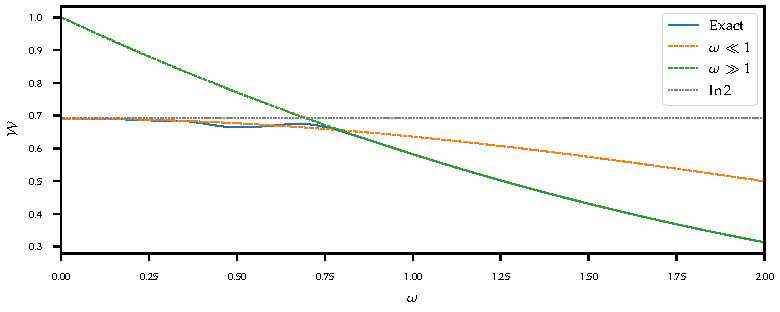
\includegraphics{figs/ergo_calc/ergo_numeric}
  \caption{\label{fig:numeric_n_ho_ergo} Numerical evaluation of
    \cref{eq:many_ho_pass} and the estimates
    \cref{eq:many_ho_ergo_bound,eq:ergo_esti_high_t} for \(N=110\)
    and \(β=1\). Good agreement can be found and the bound
    \(β^{-1}\ln2\) is approximately saturated.}
\end{figure}

In conclusion, we have found an upper bound
\cref{eq:many_ho_ergo_bound} for and a high temperature estimate
\cref{eq:ergo_esti_high_t} of the ergotropy to \(N\) oscillators in a
thermal state and a two level system in a pure state. The bound
\cref{eq:thermo_ergo_bound_specific} on ergtropy is still valid and
also tightest in the infinite bath case with vanishing level distance
\(ω\to 0\). These conditions are fulfilled for the baths usually
considered in open quantum systems, where a continuum of frequencies
are present instead of a single, very degenerate one. The energy level
distance vanishes in this case.

Even for finitely many oscillators the ergtropy bound can be
approached rather closely for finite \(ω\) as can be seen in
\cref{fig:numeric_n_ho_ergo_nonmon}. Remarkably, the ergotropy becomes
a non-monotonous function of the level spacing \(ω\) for larger \(N\)
even though there is no additional energy scale present to warrant a
resonance phenomenon.  It is always increasing with \(N\).

Also, for large \(N\) the transition into the region where the upper
bound \cref{eq:thermo_ergo_bound} is tight is very close to the
crossing point of this bound with the \(ω\ll 1\) estimate. This bound
is very tight as may be expected, because the error one makes in
\cref{eq:manhoergoestimate} becomes negligible in the case \(N\gg 1\).
\begin{figure}[htp]
  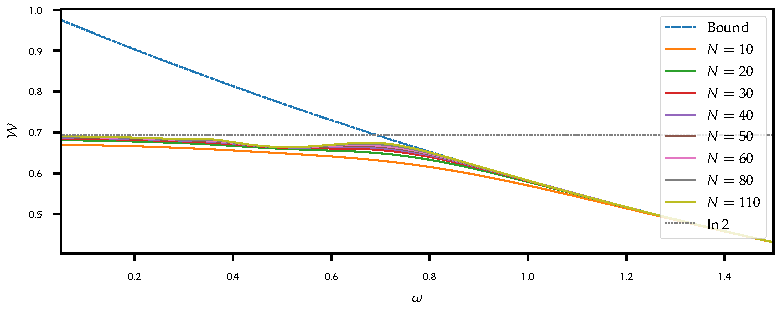
\includegraphics{figs/ergo_calc/ergo_nonmonotonic}
  \caption{\label{fig:numeric_n_ho_ergo_nonmon} Numerical evaluation of
    \cref{eq:many_ho_pass} for different \(N\) and \(β=1\).}
\end{figure}


\subsection{A bound on the Energy Change of Multiple Baths in the
  Periodic Steady State}
\label{sec:operational_thermo}
The above discussions do not apply to the more interesting case of a
system coupled to multiple independent baths of differing
temperatures. Naturally, the ergotropy of such a system cannot be
expected to be bounded in the infinite bath limit. Instead, as in
standard thermodynamics, we wish to find some limit to the amount of
energy that can be extracted out of the system in relation to the
energy that is simply transferred between the baths.

An argument based on entropy may be made for the periodic steady state
as was shown in~\cite{Kato2016Dec} and is reproduced here with the
slight generalization of multiple baths and modulated coupling. We
will find a Clausius like form of the second law. The left hand side
of this inequality can then be interpreted as thermodynamic cost of
the cyclical process.

We consider a situation specified by a Hamiltonian for a system
coupled to multiple baths under periodic driving
\begin{equation}
  \label{eq:katoineqsys}
  H(t) = H_\sys(t) + ∑_i \qty(H_\bath^i + H_\inter^i(t)).
\end{equation}
Here, \(H_\sys(t)\) is the system Hamiltonian, \(H_\bath^i\) is the
Hamiltonian of the \(i\)-th bath and \(H_\inter^i(t)\) is the coupling
to this bath. Again, the bath must be treated as finite during the
derivation.

The von Neumann entropy \(S(t)=-\tr[ρ\ln ρ]\) of the global state
whose evolution is generated by \cref{eq:katoineqsys} is
constant. Additionally it is sub-additive meaning
\begin{equation}
  \label{eq:subadd}
  S(t) \leq -\tr[ρ_\sys(t)\ln ρ_\sys(t)] - ∑_i\tr[ρ_{\bath^i}(t)\ln
  ρ_{\bath^i}(t)] \equiv S_\sys(t) + ∑_iS_{\bath^i}(t),
\end{equation}
where \(ρ_{\sys}(t)=\tr_{\bigotimes_i{\bath^i}}[ρ(t)]\) and
\(ρ_{\bath^i}=\tr_{\sys\bigotimes_{j\neq i}{\bath^j}}[ρ(t)]\) are the
marginal states of system and the \(i\)th bath respectively. Note that
the marginal entropies \(S_{\sys},\,S_{\bath}\) are generally
\emph{not} constant in time.

This implies for \(ΔS_\sys(t)\equiv S_\sys(t) - S_\sys(0)\) and
\(ΔS_{\bath^i}(t)\equiv S_{\bath^i}(t) - S_{\bath^i}(0)\)
\begin{equation}
  \label{eq:deltagreat}
  ΔS_\sys(t) + ∑_i ΔS_{\bath^i}(t) \geq 0.
\end{equation}

The von Neumann entropy of a single bath can be expressed as
\begin{equation}
  \label{eq:bathentro}
  \begin{aligned}
  S_{\bath^i}(t) &=-\tr[ρ_{\bath^i}(t)\ln ρ_{\bath^i}^β] -
                   \qty(\tr[ρ_{\bath^i}\ln ρ_{\bath^i}(t)] -
                   \tr[ρ_{\bath^i}(t)\ln ρ_{\bath^i}^β])\\
                 &= β E_{\bath^i}(t) - βF_{\bath^i} - \qrelent{ρ_{\bath^i}(t)}{ρ_{\bath^i}^β},
  \end{aligned}
\end{equation}
where
\(E_{\bath^i}(t)=\tr[ρ_{\bath^i}(t)H_{\bath^i}]=\tr[ρ(t)(H_{\bath^i}\otimes
\id)]\), \(ρ_{\bath^i}^β=\exp(-β H_{\bath^i})/Z\) and
\(F_{\bath^i}=-\ln(Z_{\bath^i})/β\) is the equilibrium free energy of
the bath at (as yet undetermined) inverse temperature \(β\).

The result \cref{eq:bathentro} implies
\begin{equation}
  \label{eq:bathenergychange}
  ΔS_{\bath^i}(t) = β_i ΔE_{\bath^i}(t) -
  \qrelent{ρ_{\bath^i}(t)}{ρ_{\bath^i}^{β_i}} \leq β_i ΔE_{\bath^i}(t).
\end{equation}
Note that \(β_i\) is now being fixed through
\(\qrelent{ρ_{\bath^i}(0)}{ρ_{\bath^i}^{β_i}}=0\Leftrightarrow
{ρ_{\bath^i}(0)}={ρ_{\bath^i}^{β_i}}\).

Combining \cref{eq:bathenergychange,{eq:deltagreat}} yields
\begin{equation}
  \label{eq:bathenergyandsystementro}
  ΔS_\sys(t) + ∑_iβ_i ΔE_{\bath^i}(t) \geq 0.
\end{equation}
This inequality only contains quantities that can be expected to be
finite, even in the limit of infinite baths.

As in \cref{sec:ergoonebath} we now demand periodic driving, that is
\(H(t+τ) = H(t)\) for some \(τ\geq 0\). Now we \emph{assume} that the
system enters a periodic steady state after the time \(n_0τ\) for some
\(n_0\in\NN\) so that \(ρ_\sys((n + n_0)τ)= ρ_\sys(n_0τ)\) for all
\(n\in\NN\). This assumption is linked to the notion of a ``finite
memory'' of the baths which implies an infinite bath\footnote{Or, as
  we have remarked earlier, a suitably large bath.}. In the same
spirit, we \emph{assume} that the energy change of each bath
\(ΔE_{\bath^i}^\cyc =ΔE_{\bath^i}((n+1)τ)-ΔE_{\bath^i}(nτ) =
E_{\bath^i}((n+1)τ)-E_{\bath^i}(nτ)\) is constant once the system is
in the periodic steady state. This behavior, at least on the system
level, is suggested by the NMQSD equation \cref{{eq:multinmqsd}}.

As the system entropy does not change over a cycle
\(ΔS_\sys^\cyc = ΔS_\sys(τ (n+n_0)) - ΔS_\sys(τ n_0)=S_\sys(τ (n+n_0)) - S_\sys(τ
n_0)=0\) vanishes and we have
\begin{equation}
  \label{eq:secondlaw_cyclic}
  ∑_iβ_i ΔE_{\bath^i}^\cyc \geq 0,
\end{equation}
as otherwise the inequality \cref{eq:bathenergyandsystementro} would
be violated in finite time.

In fact, the requirement that \(ΔE_{\bath^i}^\cyc\) be constant can be
relaxed, as \cref{eq:secondlaw_cyclic} holds as soon as
\(ΔS_\sys^\cyc\) vanishes.

The left hand side could be called ``bath entropy production'' as is
motivated in \cite{Riechers2021Apr}, where heat is identified with
\(ΔE_{\bath^i}\). There the entropy production bound
\cref{eq:bathenergyandsystementro} that takes into account system and
bath is being considered and brought into connection with
information-theoretic quantities.

If one defines heat as is done in
\cite{Kato2016Dec,Riechers2021Apr,Strasberg2021Aug} as the change of
bath energy, \cref{eq:secondlaw_cyclic} amounts to the Clausius form
of the second law. This definition of heat is corroborated
in~\cite{Esposito2015Dec} where it is shown\footnote{for fermionic
  baths} that a definition of heat involving any nonzero fraction of
the interaction energy will lead to the internal energy (as defined by
the first law) not being an exact differential.

In contrast to~\cite{Strasberg2021Aug}, no interpretation in terms of
thermodynamical quantities is required for \cref{eq:secondlaw_cyclic}
to be useful.  Assume that the interaction Hamiltonian in
\cref{eq:katoineqsys} vanishes periodically, so that system and bath
energy expectation values can be cleanly separated. In the periodic
steady state the system energy does not change during a cycle and the
whole energy change amounts to the change in bath energy. In a setting
with two baths \cref{eq:secondlaw_cyclic} implies the Carnot bound for
the efficiency given in \cref{eq:efficiency_definition}.

\section{Modulation of System and Interaction for a Single Bath}
\label{sec:singlemod}
Because the HOPS method is best suited to situations where the actual
finite time dynamics are of interest, let us now turn to such a
problem.

A classical dictum of thermodynamics is, that it is impossible to
extract energy from a single bath in a cyclical manner. Indeed, we
found in \cref{sec:ergoonebath} that this also holds for a finite
quantum system coupled to a thermal bath. In \cref{sec:explicitergo}
we found, that the bound given on the ergotropy in such a situation
can be saturated for infinite baths, such as the ones used with
NMQSD/HOPS. However, it is unclear if such a unitary transformation
can be implemented without explicit construction of a model. Our goal
in this section is to extract as much energy from a one-bath system as
is possible without extensive tuning. We will applying the results of
the previous studies of \cref{chap:numres} to produce consistent
results.

In this section we will focus on the minimal dimensionless model
\begin{equation}
  \label{eq:one_qubit_model_driven}
  H = \frac{1}{2} \bqty{(σ_z+1)+λΔ \sin(Δτ) σ_{f}} + \frac{1}{2}
  {\sin[2](\frac{Δ}{2}τ)} ∑_λ\qty(g_λ σ_x^† a_λ + g_λ^\ast
  σ_x a_λ^†) + ∑_λ ω_λ a_λ^\dag a_λ,
\end{equation}
where \(λ,Δ\geq 0\) and \(f\in \{z, y\}\). The form of the system
Hamiltonian has been chosen similar to \cite{Mukherjee2020Jan}, where
Floquet theory was used, and it was shown that the relevant quantities
are scaling with \(λ\). For \(λ=0\) the system Hamiltonian is positive
semi-definite with the energies zero and one.  The modulation of the
interaction has been chosen heuristically to always act in the same
``direction'' and vanish periodically. We choose the ``down state''
with \(H(0)\ket{0}=0\) as initial state, as we want to extract energy
from the bath and not the system. To maximize energy flow, we will use
resonant baths whose spectral densities have been shifted such that
their maxima coincide with \(1 + Δ\).

Despite the simplicity of the model \cref{eq:one_qubit_model_driven}
simplicities there too many free parameters. We will narrow down the
field of possible paramteres in
\cref{sec:quantum_friction,sec:sys_mod_v_no_sys_mod} and then focus on
the energy extraction performance in relation to properties of the
bath and the modulation frequency in
\cref{sec:extr_mem,sec:speedlim,sec:modcoup_reso}.

For this model the ergotropy bound \cref{eq:ergo_bath_change}
evaluates to
\begin{equation}
  \label{eq:ergo_mod_model}
  \mathcal{W} \leq β^{-1} \ln(1+\eu^{-β})=\mathcal{W}_{\mathrm{max}}.
\end{equation}
For \(β\to ∞\) we find \(\mathcal{W} = 0\) as the temperature \(T\)
must be of the order of the system energy gap or larger for any energy
lowering process to take place.

\subsection{Quantum Friction}
\label{sec:quantum_friction}
Before focusing on the \(λ = 0\) case, we will briefly revisit the
phenomenon introduced in \cref{sec:quantum_friction_theory}. The so
called \emph{Quantum Friction} is the creation of
coherences\footnote{Or more generally the creation of ergotropy.} in
the system energy basis and hinders the performances of thermal
quantum machines. These coherences raise the ergotropy of the system
consuming that could have been extracted by the external modulation.
\begin{figure}[htp]
  \centering
  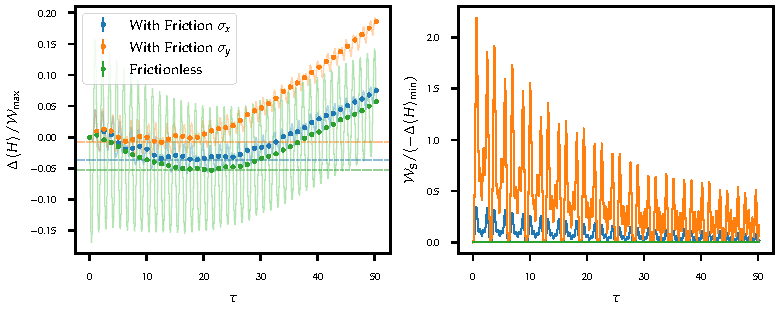
\includegraphics{figs/one_bath_mod/quantum_friction}
  \caption{\label{fig:quant_frict} Total energy change normalized by
    the maximal ergotropy in the left panel and the ergotropy of the
    system state \(ρ_{\sys}\) normalized by the maximal extracted
    energy (dashed lines in left panel) in the right panel over
    time. Here \(λ=0.1, Δ=5, T=5\) was chosen. In the ``With
    Friction'' case \(σ_{f}=σ_{x,y}\) and in the ``Frictionless'' case
    \(σ_{f}=σ_{z}\).  The solid dots mark the times when
    \(H_{\inter} = 0\). The horizontal dashed lines mark the minimal
    total energy differences achieved.  For more parameters see
    \cref{tab:plus_friction}. In the frictionless case the most energy
    is being extracted. The \(σ_{y}\) modulation that commutes neither
    with the system Hamiltonian nor with the interaction performs
    worst.}
\end{figure}

A simple demonstration of this can be observed in
\cref{fig:quant_frict}. Here the simulation with nondiagonal
modulation \(σ_{f}=σ_{x}\) does extract less energy from the total
system as the \(σ_{f}=σ_{z}\) case. One reason for this is the not
insignificant buildup of ergotropy in the system state which is being
reduced to zero periodically, but does retard the energy extraction so
that less energy is extracted before the periodic steady state is
being reached which does only increase energy as was shown in see
\cref{sec:operational_thermo}.

When choosing \(σ_{f}=σ_{y}\) the situation becomes even worse because
now the system modulation does not even commute with the
interaction. The extracted energy is smallest and the relative system
ergotropy buildup is much larger than in the \(σ_{f}=σ_{x}\) case.

\subsection{System Modulation}
\label{sec:sys_mod_v_no_sys_mod}
As it turns out, the modulation generically leads to a deterioration
of energy extraction performance for the model
\cref{eq:one_qubit_model_driven} as is demonstrated in
\cref{fig:quant_frict_sys_no_sys}. Again, the ``friction'' (system
ergotropy) generated by the system modulation is much greater than
without system modulation. However, it is questionable whether this is
the only reason for the performance advantage of the case without
system modulation. Another factor is, that the system goes in and out
of resonance with the bath and therefore hampers the interaction.
\begin{figure}[htp]
  \centering
  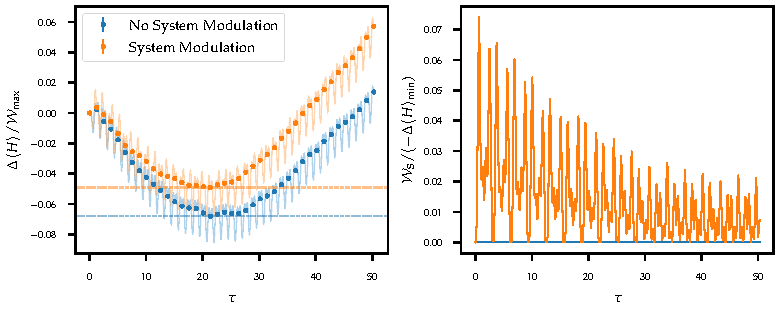
\includegraphics{figs/one_bath_mod/system_vs_no_system}
  \caption{\label{fig:quant_frict_sys_no_sys} Similar to
    \cref{fig:quant_frict}, but for (frictionless) system modulation
    and no system modulation. The parameters were
    \(λ=0.1,\, Δ=5,\, T=5\) and further details can be found in
    \cref{tab:plus_system}. Less energy is extracted when the system
    Hamiltonian is being modulated.}
\end{figure}

In light of this result we shall continue with \(λ=0\), which
simplifies the situation. An interesting question for future is
whether a phase shift in the system modulation may be able to improve
energy extraction performance.

\subsection{Energy Extraction with different Bath Memories}
\label{sec:extr_mem}
To find out whether a substantial fraction of the maximal ergotropy
can be extracted from a system we have numerically optimized the
coupling strengths of the model \cref{eq:one_qubit_model_driven}, so
that over ten modulation periods \(τ_{m} = \frac{2 π}{Δ}\) the maximal
absolute interaction energy is close to a give value (here
\(\ev{H_{\inter}}\approx 0.4\)) for various cutoff frequencies
\(ω_{c}\).
\begin{figure}[htp]
  \centering
  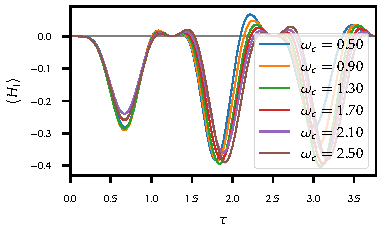
\includegraphics{figs/one_bath_mod/omega_interactions}
  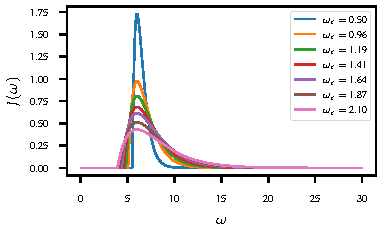
\includegraphics{figs/one_bath_mod/omega_sd}
  \caption{\label{fig:omega_couplings_and_energies} The interaction
    energies and (zero temperature) spectral densities for the
    simulations in this section. Here we used \(λ=0.1, Δ=5, T=5\) and
    the parameters in \cref{tab:plus_omega}.}
\end{figure}

The resulting interaction energies can be found in
\cref{fig:omega_couplings_and_energies}. They correspond roughly to
demanding \(α_{β}(0)=1.4\), where \(α_{β}\) is the finite temperature
bath correlation function.  \Cref{fig:omega_couplings_and_energies}
also shows that for the simulations with small \(ω_{c}\) the positive
parts of the interaction energy are especially large. This is a major
departure from the pure dephasing regime where the interaction energy
is always negative.

For very weak coupling \(\ev{H_{\inter}}\approx 0.01\)
\cref{fig:omega_couplings_weak} shows that this optimization procedure
yields the normalization of \cref{eq:normohmic} so that the peak
heights of all spectral densities coincide. For weak coupling, only
the peak value of the spectral density is important and therefore the
peaks must coincide for similar coupling strengths.

In \cref{fig:omegas_total} we see the energy extraction behaviour of
the model for various cutoff frequencies.
\begin{figure}[htp]
  \centering
  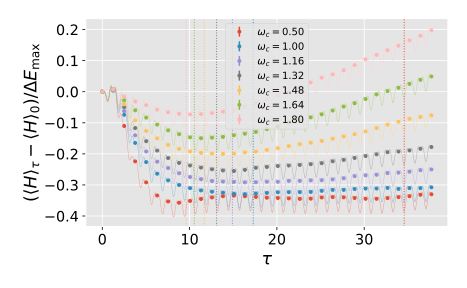
\includegraphics{figs/one_bath_mod/omegas_total}
  \caption{\label{fig:omegas_total} The total energy differences of
    \cref{eq:one_qubit_model_driven} for various \(ω_{c}\). For
    details of the parameters see
    \cref{fig:omega_couplings_and_energies}. The dots mark the times
    when the interaction is turned off.  The dashed lines show the
    position of the where the total energy is minimal. Lower cutoffs
    \(ω_{c}\) lead to more extracted energy. For \(ω_{c}=2.1\) no
    energy is being extracted.}
\end{figure}
It is clear, that a lower cutoff frequency is advantageous as the
minimal total energy is achieved earlier and is of greater
magnitude. Further, we see that a non-trivial amount of energy is
being extracted relative to the ergotropy bound
\cref{eq:ergo_mod_model}.

\begin{figure}[htp]
  \centering
  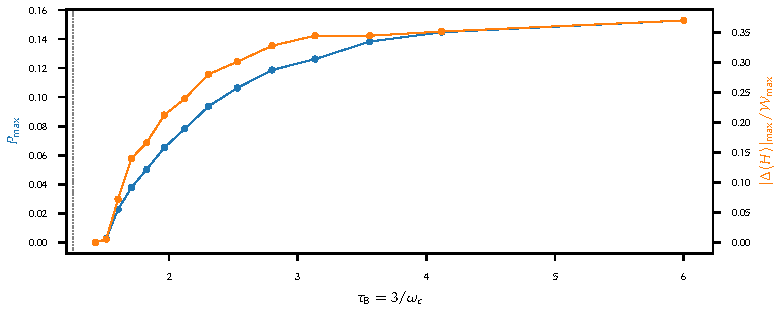
\includegraphics{figs/one_bath_mod/omega_energies_and_powers}
  \caption{\label{fig:omegas_energies_and_powers} One shot power
    (blue) and maximal extracted energy (orange) as a function of the
    bath memory. The grey vertical line marks one modulation
    period. Longer memories lead to greater energy extractions and
    greater one shot power.}
\end{figure}
\Cref{fig:omegas_energies_and_powers} shows that longer bath memories,
defined as the time point at which \(α(τ_{\bath}) = α(0)/10\), lead to
both increased energy extraction and increased one shot power. The one
shot power is defined as
\begin{equation}
  \label{eq:one_shot_power}
  P_{\max}=\max_{n\in\NN}\frac{\abs{Δ\ev{H}_{n τ_{m}} \cdot Θ(-Δ\ev{H}_{n τ_{m}})}}{n τ_{m}},
\end{equation}
where \(Δ\ev{H}_{τ}= \ev{H}_{τ} - \ev{H}_{0}\) and \(Θ\) is the
Heaviside function.  The concrete shape of the curve
\cref{fig:omegas_energies_and_powers} is hard to discuss because of
the nontrivial shape and magnitude of the spectral densities. However,
the abrupt transition to zero for short memories is due to the
requirement that power and extracted energy have to be positive, and
the stroboscopic time view induced by the requirement that the
interaction energy should be zero.

It can be concluded that in the cases studied here we can extract a
finite amount of energy from the system as soon as the bath memory is
somewhat longer than the modulation period. This statement depends on
the definition of the memory time \(τ_{\bath}\) and therefore be taken
as a rule of thumb.

\subsection{Modulation Frequency and Speed Limit}
\label{sec:speedlim}
Another interesting parameter to tune is the modulation frequency
\(Δ\), or equivalently the modulation period time \(τ_{p}=2π/Δ\). In
driven systems, there usually appears a ``quantum speed
limit''~\cite{Kurizki2021Dec} that limits the power output of a driven
system at a given coupling strength. An example is the transition from
engine to refrigerator in a continuously coupled two-bath engine in
\cite{Mukherjee2020Jan}. More generally, this issue is connected to
non-adiabatic changes in the Hamiltonian that can generate non-passive
states \cite{Binder2018}.

Intuitively speaking, slower modulation allows more time for the
system-bath interaction that enables energy extraction from the
initially passive bath state in the first place.

The continuous power is given by
\begin{equation}
  \label{eq:power_for_onequbit}
  P = \ev{\dot{H}_{\inter}} \sim Δ \sin(Δ) \ev{B σ_{x}^{†} + \hc},
\end{equation}
where \(H_{\inter, m} \equiv \ev{B σ_{x}^{†} + \hc}\) constitutes the
unmodulated interaction Hamiltonian. Increasing the frequency \(Δ\)
will increase the amplitude of \cref{eq:power_for_onequbit}. On the
other hand, if the expectation value of \(H_{\inter, m}\) does not
change much or on a much slower scale than \(τ_{p}\) because of too
fast modulation, the \(Δ\sin(Δ)\) factor will cause the expression to
average out to zero (Zeno-like effect,~\cite{Kurizki2021Dec}).

Stronger coupling will lead to a greater expectation value of
\(H_{\inter, m}\) and generically to more power in the region in
parameter space we are going to explore.

To assess the behaviour with regard to coupling and modulation speed,
we simulated the model for \(ω_{c}=1\) up to the time \(τ=20\) and
plotted the one shot power \cref{eq:one_shot_power} in a heatmap in
\cref{fig:power_heatmap}. The coupling strength is quantified by the
value of the thermal bath correlation function \(α_{β}\) a time
zero. This balances the shifting of the spectral density for the
different values of \(Δ\).
\begin{figure}[htp]
  \centering
  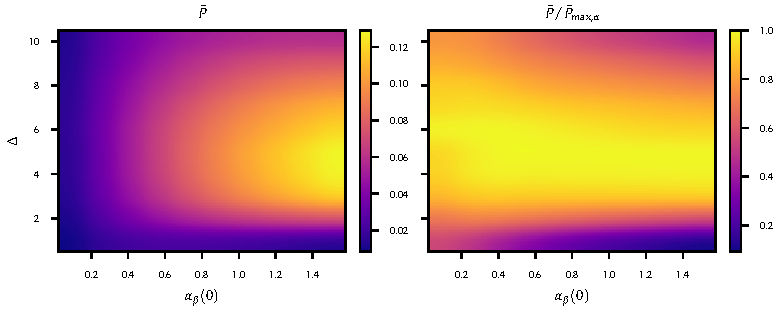
\includegraphics{figs/one_bath_mod/power_heatmap}
  \caption{\label{fig:power_heatmap} Left panel: The one shot power
    \cref{eq:one_shot_power} for the model
    \cref{eq:one_qubit_model_driven} for various modulation
    frequencies \(Δ\) and coupling strengths. The parameters
    \(ω_{c}=1,λ=0.1, T=5\) were used. Right panel: The same, but
    normalized to the maximum power for each \(α_{β}(0)\). In both
    cases \(100\) grid points and Gaussian interpolation have been
    used. The power output generally increases with the coupling
    strength, but the optimal modulation frequency becomes more
    sharply defined (right panel).}
\end{figure}
\begin{figure}[htp]
  \centering
  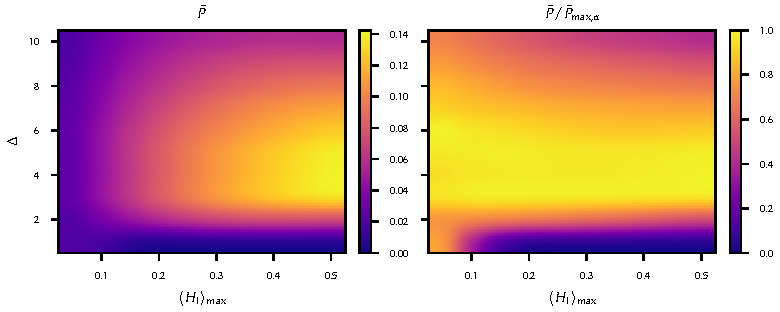
\includegraphics{figs/one_bath_mod/power_en_heatmap}
  \caption{\label{fig:power_heatmap_tuned} Like
    \cref{fig:power_heatmap_tuned} but as function of maximal
    interaction energy as in \cref{sec:extr_mem}.  The parameters of
    the underlying simulations can be found in
    \cref{tab:plus_mod_en}. A broadly similar behaviour to
    \cref{fig:power_heatmap} can be observed.}
\end{figure}

We find that the best power output is achieved by stronger
coupling. The dependence on the modulation frequency is more
nuanced. If the power output is normalized by its maximum value for
each \(α_{β}(0)\) it can be seen, that the optimal power output is
achieved at roughly the same modulation frequency. However, with
increasing coupling strength, the system becomes more sensitive to the
modulation frequency, exhibiting a clear maximum. This constitutes the
``speed limit'' discussed above.

Running the simulations with a peak interaction energy target like in
\cref{sec:extr_mem} the results are broadly similar on the level of
detail available to us as can be ascertained from
\cref{fig:power_heatmap_tuned}. For the \(Δ=1\) case the optimization
was generally not very effective in the weaker coupling regime as is
quantified in \cref{fig:interaction_tuning_success}. Therefore this
region should be interpreted with care.

The above results have to be taken with a grain of salt however. The grid
resolution of 10 by 10 does not allow us to perceive a shift in the
optimal modulation frequency. Also, the range of interaction strengths
is rather limited.


\begin{figure}[htp]
  \centering
  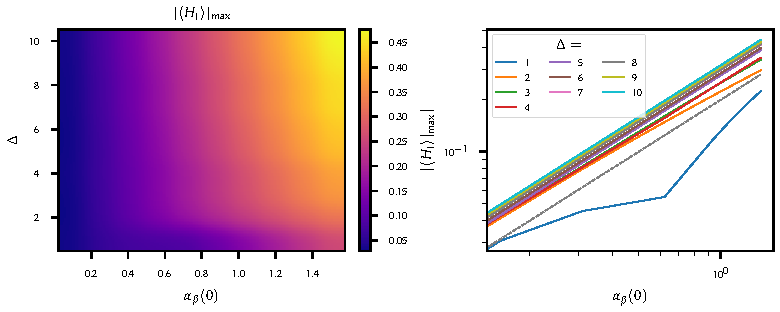
\includegraphics{figs/one_bath_mod/interaction_nontuned}
  \caption{\label{fig:interaction_nontuned} Left panel: Similar to
    \cref{fig:power_heatmap} but showing the maximal absolute
    interaction energies. Right panel: A log-log-plot of the maximal
    interaction energy over the coupling strength. The dashed grey
    line is a linear reference curve.}
\end{figure}

The maximal absolute interaction energies are shown in
\cref{fig:interaction_nontuned} for the non-optimized case of
\cref{fig:power_heatmap} and increase generally with increasing
coupling strength. The dependence on the coupling strength is linear
for modulations with \(Δ\geq 5\) but deviates for slower
modulation. This may be due to the fact, that fewer modulation periods
can be completed in the given time frame.

The interaction energy also increases for faster modulation,
especially at greater coupling strengths. Comparing
\cref{fig:interaction_nontuned} with \cref{fig:power_heatmap} we see
that the top right region where the interaction energy is strongest
somewhat coincides with a decrease in power. In this region, the
dependence of the interaction energy on the modulation frequency is
also most pronounced.  The \(Δ=1\) case is an outlier as we already
noted above and should therefore be interpreted with care. It is
likely that not enough cycles have been simulated to judge this case
accurately.

Summarizing, we found that the one shot power output for the model
\cref{eq:one_qubit_model_driven} has a complex dependence on the
coupling strength and the modulation frequency. Especially for strong
coupling, the modulation frequency has to be chosen carefully if
optimal energy extraction is desired.

\subsection{Resonance Behaviour of the One Shot Power}
\label{sec:modcoup_reso}
Finally, after having introduced the shift of the spectral density on
a rather vague basis, we would like to give a short example of its
validity.

To this end we choose the spectral densities with their peaks
slightly shifted away from \(1+Δ\) to \(1+Δ+δ\) and normalized so that
their peak height is fixed.
\begin{figure}[htb]
  \centering
  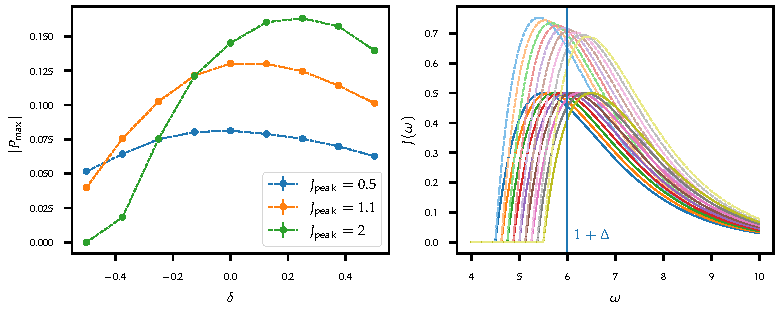
\includegraphics{figs/one_bath_mod/modulation_tuning}
  \caption{\label{fig:modulation_tuning} Left panel: The one shot
    power \cref{eq:one_shot_power} normalized for multiple values of
    the detuning \(δ\) and two peak heights. Right panel: The spectral
    densities for the peak height \(J_{\mathrm{peak}} = 0.5\). The
    dotted lines are the positive frequency parts of the effective
    finite temperature spectral density. The detailed model and
    simulation parameters can be found in \cref{tab:plus_tune}.}
\end{figure}

\Cref{fig:modulation_tuning} shows the result. In all cases, the one
shot power \cref{eq:one_shot_power} as a function of \(δ\) exhibits a
clear maximum which demonstrates the resonance effect.

For the stronger coupling case we find in \cref{fig:modulation_tuning}
that the optimal peak position has moved slightly to the right.  Note
also that even though the finite temperature spectral density
decreases in magnitude for positive shifts so that the observed
behaviour nontrivial. Also, the penalty for being off resonant in the
negative \(δ\) direction is much more severe than in the weaker case.

An explanation may be, that higher harmonics like \(1+ 2 Δ\) become
important for stronger coupling. Shifting the spectral density
slightly to higher frequencies then optimizes the resonance with those
harmonics.

\section{Quantum Otto Cycle}
\label{sec:otto}
To exploit the whole range of capabilities of the NMQSD and HOPS we
now turn to a model with multiple baths of different
temperatures. This also provides us with an opportunity to demonstrate
the usefulness and validity of the considerations of
\cref{sec:operational_thermo}, namely the bound on extractable energy
per cycle and efficiency, as well as the cost measure introduced there.

A demonstration of a standard thermodynamic cycle that is a popular
model in the literature\footnote{see
  \cite{Wiedmann2021Jun,Karimi2016Nov,Binder2018}}  is a quantum heat
engine that inspired by the Otto cycle. Similar to expansion and
compression of an ideal gas, we modulate the level spacing of our
working medium. This model serves as a good demonstration of HOPS'
capabilities in terms of being a method that can treat various bath
correlation functions and \emph{arbitrary} modulation system and
coupling.

Here, we consider a spin boson model much like the one in
\cref{sec:singlemod} but with two baths
\begin{equation}
  \label{eq:otto_model}
  H = \frac{1+f(t)}{2} (σ_z+1) +
   ∑_{i\in\{h, c\}}\bqty{h_{i}(t) ∑_λ\frac{1}{2}\qty(g_{λ,i} σ_x^† a_{λ,i} + g_{λ,i}^\ast
  σ_x a_{λ,i}^†) + ∑_λ ω_{λ,i} a_{λ,i}^\dag a_{λ,i}.}
\end{equation}

The modulation functions \(f\) and \(h_{i}\) are periodic and
constructed out of smoothstep\footnote{see \cref{sec:smoothstep}}
functions similar to \cite{Wiedmann2021Jun}.  Rather than giving the precise formulas, we instead plot
all the modulations over one period in \cref{fig:ottomod}.
\begin{figure}[htp]
  \centering
  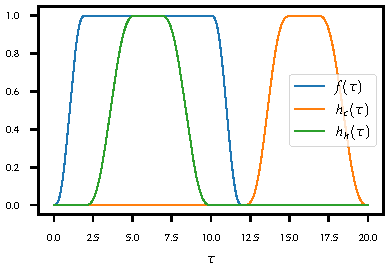
\includegraphics{figs/otto/modulation}
  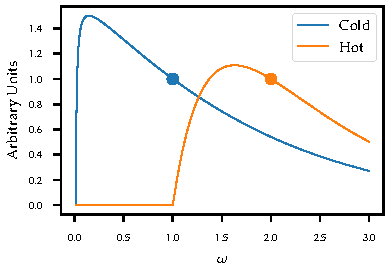
\includegraphics{figs/otto/spectral_densities}
  \caption{\label{fig:ottomod} Left panel: One period of the modulation functions
    in \cref{eq:otto_model}. Right panel: The spectral densities of
    the hot and cold baths. The dots mark the level spacing of the
    system Hamiltonian in the cold and hot phase.}
\end{figure}

First, the energy gap is widened from one to two (widening
stroke). After this, the system is coupled to a hot bath to ``charge''
for some time and decoupled before the energy gap is being compressed
from two to one again (narrowing stroke). Finally, the qubit is being
``reset'' by shedding energy into a low temperature bath.

The effective finite temperature spectral
densities\footnote{see \cref{eq:finite_bcf}} with \(ω_{c}=1\) have
been shifted so that their value is maximal for a given temperature
at the frequency of the system in its compressed (cold) or expanded
(hot) state. Their magnitudes have been chosen so that their values at
these points are the same as can be seen in \cref{fig:ottomod}.

We initialize the system in the \(H_{\sys}\ket{0}=0\) state.  For this
demonstration we chose \(T_{c}=1\) and \(T_{h}=20\) so that both
temperatures are finite but not so high that an unreasonable number of
samples is required for convergence. The interaction strength has been
chosen to be relatively weak for the same reason and to be closer to
the known weak coupling realm.

In comparison to the system timescale, the modulation cycle is rather
slow. On the other hand, the time scales on which \(f\) and \(h_{i}\)
change are not adiabatic.

\begin{figure}[htp]
  \centering
  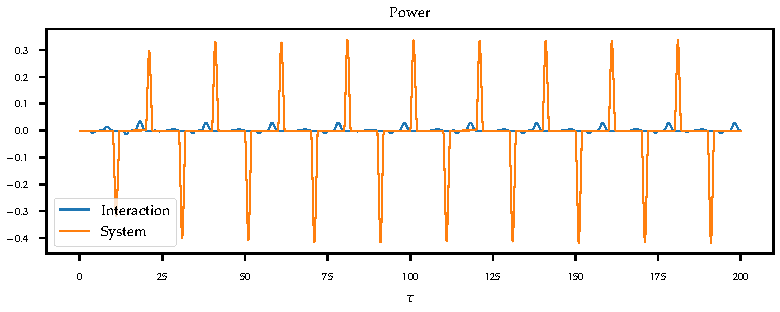
\includegraphics{figs/otto/power}
  \caption{\label{fig:ottopower} The power due to the system and the
    bath modulation of the Otto cycle model \cref{eq:otto_model}. The
    total power is
    \(\ev{\dot{H}} = \ev{\dot{H}_{\sys}} +
    \ev{\dot{H}_{\inter}}\). The interaction power is not negligible
    and in this case generally detrimental to the performance.}
\end{figure}
\Cref{fig:ottopower} shows the power due to the modulation of the
system and the interaction Hamiltonians, where the major contribution
to the total power is the system. The narrowing stroke produces
negative (usable) power and the widening produces positive power that
has to be supplied externally. More importantly however, we find that
also the modulation of the interaction, i.e. the coupling and
decoupling produce predominantly positive power that reduces the
energy output. In a weak coupling scheme, this contribution can be
neglected. Not so however in the generic case presented here. A
similar result was arrived at in \cite{Wiedmann2021Jun}.

The mean power output of this cycle is
\(\bar{P}=0.002468\pm 0.000021\) with an efficiency, as defined in
\cref{eq:efficiency_definition}, of \(η=29\%\).

Neglecting the energy change due to the coupling modulation we find
instead \(\bar{P}=0.004337\pm 0.000018\) and \(η=52\%\).  This
efficiency is, likely coincidentally, close to the efficiency given in
\cite{Geva1992Feb} for the quantum Otto cycle under quasistatic
modulation. In any case we are quite far from the Carnot efficiency
for the given temperatures \(η_{c}=95\%\).

\begin{figure}[htp]
  \centering
  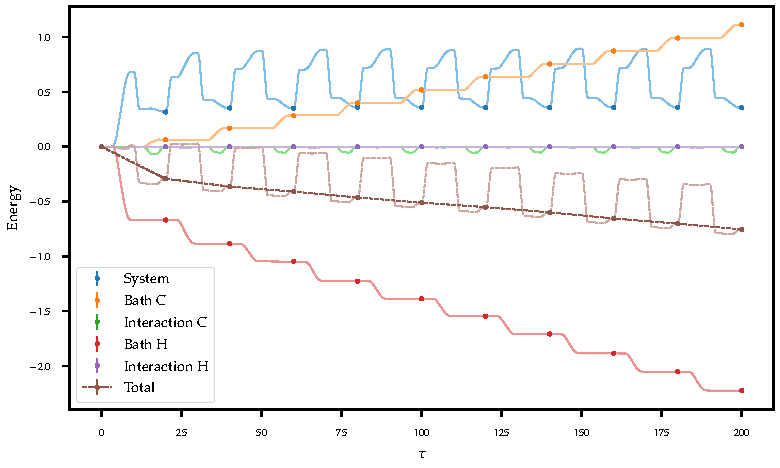
\includegraphics{figs/otto/energy_strobe}
  \caption{\label{fig:ottoenergy} The system, bath and interaction
    energies as well as the total energies of the model
    \cref{eq:otto_model}. The dots mark the times where one cycle is
    completed.}
\end{figure}
In \cref{fig:ottoenergy} we show the full energy dynamics. The
interaction energy for the coupling to the hot bath is almost
negligible, while the interaction with the cold bath is stronger. The
system energy change due to the both is of similar magnitude, however.
A periodic steady state is reached after roughly two cycle periods. In
this steady state, the system and interaction related quantities are
constant in the stroboscopic view (the dots in \cref{fig:ottoenergy}),
while the total energy and the bath energies depend linearly on
time. The assumptions of \cref{sec:operational_thermo} are being met
precisely.

We do not see oscillations in the bath energy which would
indicate the more complicated energy transfer behaviour we found in
\cref{sec:one_bath_cutoff}, signifying that we are working in a rather
``tame'' regime as intended.

The Gibbs like inequality \cref{eq:secondlaw_cyclic} derived in
\cref{sec:operational_thermo} can also be verified in this case.
We find
\begin{equation}
  \label{eq:secondlaw_otto_actual}
  ∑_iβ_i ΔE_{\bath^i}^\cyc = 0.1096\pm 0.0008 ≥ 0,
\end{equation}
which does satisfy the inequality to over 100 standard
deviations. Minimizing this dimensionless quantity maximizes the
efficiency.

With this cycle, little coherence is generated\footnote{see
  \cref{eq:otto_coherences}} leading so called ``frictionless''
dynamics. See also \cref{eq:otto_bloch} for a plot of the trajectory
of the system density matrix in the bloch sphere.

Because it requires little additional effort, we can briefly explore a
continuously coupled version off this model, where the coupling
modulation is switched off, and we thus have \(h_{1}(τ)=1\). We find
in \cref{fig:ottoenergy_cont} that work extraction is still possible,
albeit at a much lower power output \(\bar{P}=0.001670\pm 0.000029\)
and efficiency \(η=5\%\).
\begin{figure}[htp]
  \centering
  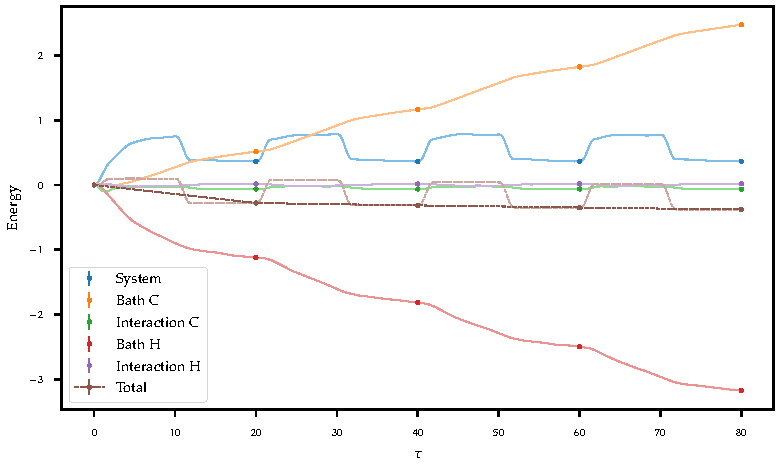
\includegraphics{figs/otto/energy_strobe_continuous}
  \caption{\label{fig:ottoenergy_cont} The system, bath and
    interaction energies as well as the total energies of the model
    \cref{eq:otto_model} for continuously coupled baths. The dots mark
    the times where one cycle is completed. We can observe positive
    energy extraction albeit at a much reduced power
    \(\bar{P}=0.001670\pm 0.000029\) and efficiency \(η=5\%\) compared
    to the modulated case in \cref{fig:ottoenergy}.}
\end{figure}

The finite energy extraction is due to the baths being alternately
resonant and off-resonant. Increasing the amplitude of the system
modulation and consequently the gap between the peaks of the spectral
densities should improve the performance.

The lost efficiency is due to energy flowing ``through'' the system
unused, a behaviour which is promoted by the continuous coupling and
reflected in the entropy production
\(∑_iβ_i ΔE_{\bath^i}^\cyc = 0.6198\pm 0.0021\).

Nevertheless, if the cycle was very fast, the effect of the
(un)coupling of the baths could be so detrimental that the
continuously coupled version of the cycle is superior. See also the
remarks below about \cite{Uzdin2015Sep}.


% \section{Anti Zeno Engine}
% \label{sec:antizeno}
% \begin{itemize}
% \item mention concept
% \item results not reliable in time for thesis
% \item interesting because: non markovian QUANTUM advantage. a bit
%   sensational ;P
% \end{itemize}

\section{Some Proposals for future Work}
\label{sec:some-prop-future}
A worthwhile task for future work would be to verify the results
summarized in \cite{Binder2018} for the Otto cycle. Especially the
optimization for optimal power which leads to the
Novikov–Curzon–Ahlborn efficiency \(η_{ca}=1-\sqrt{T_{c}/T_{h}}\) is
interesting in the case of stronger coupling.

Another cycle to study would be a Carnot-type cycle, where the
modulation of the system and the thermalization with the bath occur at
the same time. Interpolating between Otto and Carnot, as well as
studying the effect of overlapping and shifting strokes is a
fascinating avenue for future exploration.

Also, more interesting working media, such as a three level system are
of interest. In \cite{Uzdin2015Sep} it is shown, that in certain
regimes quantum coherence can lead to superior power output. In the
same regime different types heat engines are equivalent. Both these
effects have been observed experimentally in \cite{Klatzow2019Mar}. It
would be interesting to see if the slight deviations from theory in
\cite{Klatzow2019Mar} could be explained using HOPS.

The so called Anti-Zeno Effect occurring in systems under fast
modulation has recently received some attention
\cite{Mukherjee2020Jan,Xu2022Mar}. An advantage is claimed to exist,
due to the broadening of the resonance criterion which we have
observed in
\cref{sec:one_bath_cutoff,sec:modcoup_reso,sec:otto}. Being a
consequence of the energy time uncertainty it is being argued, that
the origin of this advantage is truly quantum. The tools for the
exploitation of this effect and its verification are provided in this
work. However, a strong coupling analysis has already been performed
using HEOM in \cite{Xu2022Mar}.

In \cite{Santos2021Jun} a cycle is proposed that first creates states
of finite ergotropy by letting energy flow through the working medium
and then extracting this ergotropy in a separate stroke. This work
could be verified and expanded to the non Markovian regime.

A useful improvement of the method would be the ability to snapshot
the total state of system and bath and then propagate this state with
different modulation protocols.

% \begin{itemize}
% \item ... list all those nice papers ...
% \item the third law
% \item look more deeply into the peculiarities in \cref{sec:oneosccomp}
% \item verify speculation of energy flow vs non-markvianity: flow
%   between two baths though a system
% \item three level system -> paper
% \item driven spin boson -> paper \cite{Magazzu2018Apr}
% \item flows crossing in one point: robust featureu
% \item linear regeime of steady state energies -> universal, how far
%   does it extend
% \item more detailed parameter scans, universality between different models?
% \item state changes -> is energy difference = heat + work path
%   independent (maybe try different protocols and turn off interaction
%   at for beginning and end in an adiabatic way...)
% \item compare with results from master equation in \cref{sec:prec_sim}
% \item steady state methods, better convergence for long-time
%   simulations
% \item coupling to single bath: although breach of second law forbidden
%   -> cyclical energy transfer for very long bath correlation times
% \item filter mode: \cref{sec:shift_sp}
% \item otto cycle: sensitivity to timing stronger with stronger coupling?
% \end{itemize}
